\documentclass[12pt]{article}

%Formatting Libraries
\usepackage[english]{babel}
\usepackage[utf8]{inputenc}
\usepackage[autostyle, english = american]{csquotes}
\MakeOuterQuote{"}
\usepackage{listings}
\usepackage{keyval}
\usepackage{xcolor}
\usepackage{textcomp}
\usepackage{fullpage}
\usepackage{setspace}
\usepackage{graphicx}
\usepackage{hyperref}
\usepackage{verbatim}
%\usepackage[]{mcode}
\usepackage{multicol}
\usepackage{float}
\usepackage{framed}
\usepackage{parskip}
\setlength{\parindent}{15pt}
\usepackage[fleqn]{amsmath}
\usepackage{pifont}% http://ctan.org/pkg/pifont
\newcommand{\cmark}{\ding{51}}%
\newcommand{\xmark}{\ding{55}}%
\usepackage{cancel}
\usepackage{algorithm2e} % algorithms
\usepackage[most]{tcolorbox} % solution boxes
\usepackage{mdframed}
\usepackage{lipsum}

%Symbols Libraries
\usepackage[fleqn]{amsmath}
\usepackage{amssymb}
\usepackage{amsfonts}
\usepackage{amsthm}
\usepackage{marvosym}
\usepackage{wasysym}
\usepackage{slashbox}

%For Image Generation
\usepackage{tikz}
\usepackage{tkz-euclide}
\usetikzlibrary{positioning}
\usetikzlibrary{arrows}
\usepackage[toc,page]{appendix}  % Appendix package

%For Theorem Environment
\newtheorem{theorem}{Theorem}
%Theorems numbering follow section numbers
\newtheorem{definition}[theorem]{Definition}
%definitions follow the number system that theorems do
\newtheorem{lemma}[theorem]{Lemma}
\newtheorem{corollary}[theorem]{Corollary}
\newtheorem{remark}[theorem]{Remark}
\newtheorem{proposition}[theorem]{Proposition}
%lemmas & corollaries follow the same number system as theorems do

%Making shortcuts
\renewcommand\qedsymbol{$\blacksquare$}
\newcommand{\rup}[1]{\overset{\rightharpoonup}{#1}}
\newcommand{\C}{\mathbb C}
\newcommand{\Q}{\mathbb Q}
\newcommand{\F}{\mathbb F}
\newcommand{\R}{\mathbb R}
\newcommand{\Z}{\mathbb Z}
\newcommand{\N}{\mathbb N}
\newcommand{\rank}[1]{\mathrm{rank}\left({}#1\right)}
\newcommand{\ran}[1]{\text{Ran}\left({}#1\right)}
\newcommand{\diag}[1]{\text{diag}\left({}#1\right)}
\newcommand{\nullity}{\mathrm{nullity}}
\newcommand{\st}{ \ |\ }
\newcommand{\DS}{\displaystyle}
\newcommand{\RA}{\Rightarrow}
\newcommand{\LA}{\Leftarrow}
\newcommand{\LRA}{\Leftrightarrow}
\newcommand{\ip}[2]{\left\langle{}#1,#2\right\rangle{}}
\newcommand{\lip}[2]{\left({}#1,#2\right){}}
\renewcommand{\labelenumii}{\alph{enumii}.)}
\newcommand{\curly}[1]{\left\{{}#1\right\}}
\newcommand{\eps}{\varepsilon}
\newcommand{\emp}{\varnothing}
\newcommand{\ellinf}{\ell^{\infty}}
\newcommand{\inv}{^{-1}}
\newcommand{\sgn}{\text{sgn}}
\newcommand{\tr}[1]{\text{tr}\left({}#1\right)}
\newcommand{\norm}[1]{\left|\left|{}#1\right|\right|}
\newcommand{\infnorm}[1]{\left|\left|{}#1\right|\right|_{\infty}}
\newcommand{\linfnorm}[1]{\left|\left|{}#1\right|\right|_{L^{\infty}}}
\newcommand{\onenorm}[1]{\left|\left|{}#1\right|\right|_1}
\newcommand{\twonorm}[1]{\left|\left|{}#1\right|\right|_2}
\newcommand{\xnorm}[1]{\left|\left|{}#1\right|\right|_X}
\newcommand{\abs}[1]{\left|{}#1\right|}
\newcommand{\pare}[1]{\left({}#1\right)}
\newcommand{\brak}[1]{\left[{}#1\right]}
\newcommand{\red}[1]{\textcolor{red}{#1}}
\newcommand{\green}[1]{\textcolor{Green}{#1}}
\newcommand{\floor}[1]{\lfloor #1 \rfloor}
\newcommand{\ceil}[1]{\lceil #1 \rceil}
\newcommand{\tif}{\text{ if }}
\newcommand{\ve}[1]{\textbf{#1}}
\newcommand{\St}{\text{S.t. }}
\newcommand{\bmat}[1]{\begin{bmatrix} #1 \end{bmatrix}}
\newcommand{\pmat}[1]{\begin{pmatrix} #1 \end{pmatrix}}
\newcommand{\spn}{\text{span}}
\newcommand{\aut}[1]{\text{Aut}\left({}#1\right)}
\newcommand{\inn}[1]{\text{Inn}\left({}#1\right)}
\newcommand{\var}[1]{\text{Var}\left({}#1\right)}
\newcommand{\cov}[2]{\text{Cov}\left({}#1,#2\right){}}
\newcommand{\divergence}{\nabla \cdot}
\newcommand{\curl}{\nabla \times}
\newcommand{\omint}{\int_{\Omega}}
\newcommand{\tsp}{\vspace{3mm}}
\newcommand{\ul}[1]{\underline{#1}}

%To make it so that the equation number follows subsections
\numberwithin{equation}{section}

% ¯\_(ツ)_/¯
\newcommand{\shrug}[1][]{%
\begin{tikzpicture}[baseline,x=0.8\ht\strutbox,y=0.8\ht\strutbox,line width=0.125ex,#1]
\def\arm{(-2.5,0.95) to (-2,0.95) (-1.9,1) to (-1.5,0) (-1.35,0) to (-0.8,0)};
\draw \arm;
\draw[xscale=-1] \arm;
\def\headpart{(0.6,0) arc[start angle=-40, end angle=40,x radius=0.6,y radius=0.8]};
\draw \headpart;
\draw[xscale=-1] \headpart;
\def\eye{(-0.075,0.15) .. controls (0.02,0) .. (0.075,-0.15)};
\draw[shift={(-0.3,0.8)}] \eye;
\draw[shift={(0,0.85)}] \eye;
% draw mouth
\draw (-0.1,0.2) to [out=15,in=-100] (0.4,0.95); 
\end{tikzpicture}}

\begin{document}
\begin{center}
\begin{large}
Math 9830\\
Lab 1\\
Sean Ingimarson
\end{large}
\end{center}

\begin{enumerate}
\item  Come up and write down the pseudo-code to compute the product of the transpose of the $n \times n$ sparse matrix $A$ in CSR format with a vector $x$:
$$y=A^Tx$$
Do not use the naive way by searching for all non-zero entries in column $i$.  The number of operations performed in the algorithm shouild be $O(n)$ (assuming a constant number of entries by row).

\tsp

\begin{tcolorbox}[breakable]

We learned in class the pseudo-code for calculating $y=Ax$, which is given in algorithm \ref{alg:Ax}.

\begin{algorithm}[H]
\For{$i=0:n-1$}{
	$y[i]=0$\;
	\For{$idx = \text{rowstart}[i]:\text{rowstart}[i+1]-1$}{
		$y[i]+=\text{values}[idx]\cdot x[\text{columns}[idx]]$\;
	}
}
\caption{Solving $y=Ax$ in CSR}
\label{alg:Ax}
\end{algorithm}

We can think about this as running through the $x$ vector starting off at the row vectors (where $idx$ iterates through) and then indexing through the column vectors to find the $x$ entry that multiplies the corresponding $values$ entry.

Now to solve $y=A^Tx$ while saving the exact same $rowstart$, $columns$, and $values$ vectors, we would like to swap the location of the $columns$ vector check for $y$ and $x$.  It's intuitive to think this way because the rows and columns are very literally being swapped.  The pseudo-code is described in algorithm \ref{alg:A^Tx}.

\begin{algorithm}[H]
\For{$i=0:n-1$}{
	$y[i]=0$
}
\For{$i=0:n-1$}{
	\For{$idx = \text{rowstart}[i]:\text{rowstart}[i+1]-1$}{
		$y[\text{columns}[i]]+=\text{values}[idx]\cdot x[idx]$\;
	}
}
\caption{Solving $y=A^Tx$ in CSR}
\label{alg:A^Tx}
\end{algorithm}
Note we also initialize the $y$ vector as a row of zeros to start off with because we will call on other values of $y$ throughout the new algorithm, so initialization is necessary.  The output is visible in problem 3, figure \ref{fig:Screenshot}.
\end{tcolorbox}

\item Take a look at the \texttt{01\_sparse\_mat} source code from the class repo and implement your pseudocode in 1) in the function \texttt{mat\_vec\_transposed}.  Submit your \texttt{main.cc} solution on Canvas.

\begin{tcolorbox}[breakable]
The code verbatim is copied directly from Qt Creator on Linux:

\begin{verbatim}
  void mat_vec_transposed(Vector &dest, const Vector &src)
  {
      for (int i=0; i<n; ++i)
      {
          dest.values[i]=0.0;
      }
      for (int i=0; i<n; ++i)
        {
          for (int idx=row_start[i]; idx<row_start[i+1]; ++idx)

            dest.values[column_indices[idx]] += values[idx]*src.values[i];
        }
  }
\end{verbatim}
\end{tcolorbox}


\item Take a look at the function \texttt{print\_full} in the same program: notice that the output is incorrect (see the last intry in the second row).  Try to fix this bug.

\begin{tcolorbox}[breakable,enhanced]
The code is copied directly from Qt Creator:

\begin{verbatim}
   void print_full()
  {
    for (int r=0; r<n; ++r)
      {
        int idx = row_start[r];
        for (int c=0; c<n; ++c)
          {
            if (c > column_indices[idx])
              ++idx;
            if (c == column_indices[idx])
              std::cout << values[idx] << "\t";
            else
              std::cout << "-\t";
          }
        std::cout << std::endl;
      }
  }
\end{verbatim}

Upon inspection of the code and the output, this function outputs the following matrix:
$$\bmat{1.1 & - & - & -1.5\\ 1.2&2&-&5.5\\-&-&-&5.5\\-&-&1.3&-}$$
The issue here is that there is an extra 5.5 in the $(1,3)$ position.  This tells us there is something wrong with the way the values are being called, in other words $idx$ is not being iterated correctly.  This should lead us right to the if statement where $c>col[idx]$ is being considered.

Coming from a theory perspective, we should notice that idx needs to stop iterating once it reaches it's iteration limit, which is \texttt{row\_start[r+1]-1}.  So we implement a check to make sure idx is not too large.  We change the if statement to the following:
\begin{verbatim}
            if (c > column_indices[idx] && idx < row_start[r+1]-1) 
              ++idx;
\end{verbatim}


\begin{figure}[H]
\centering
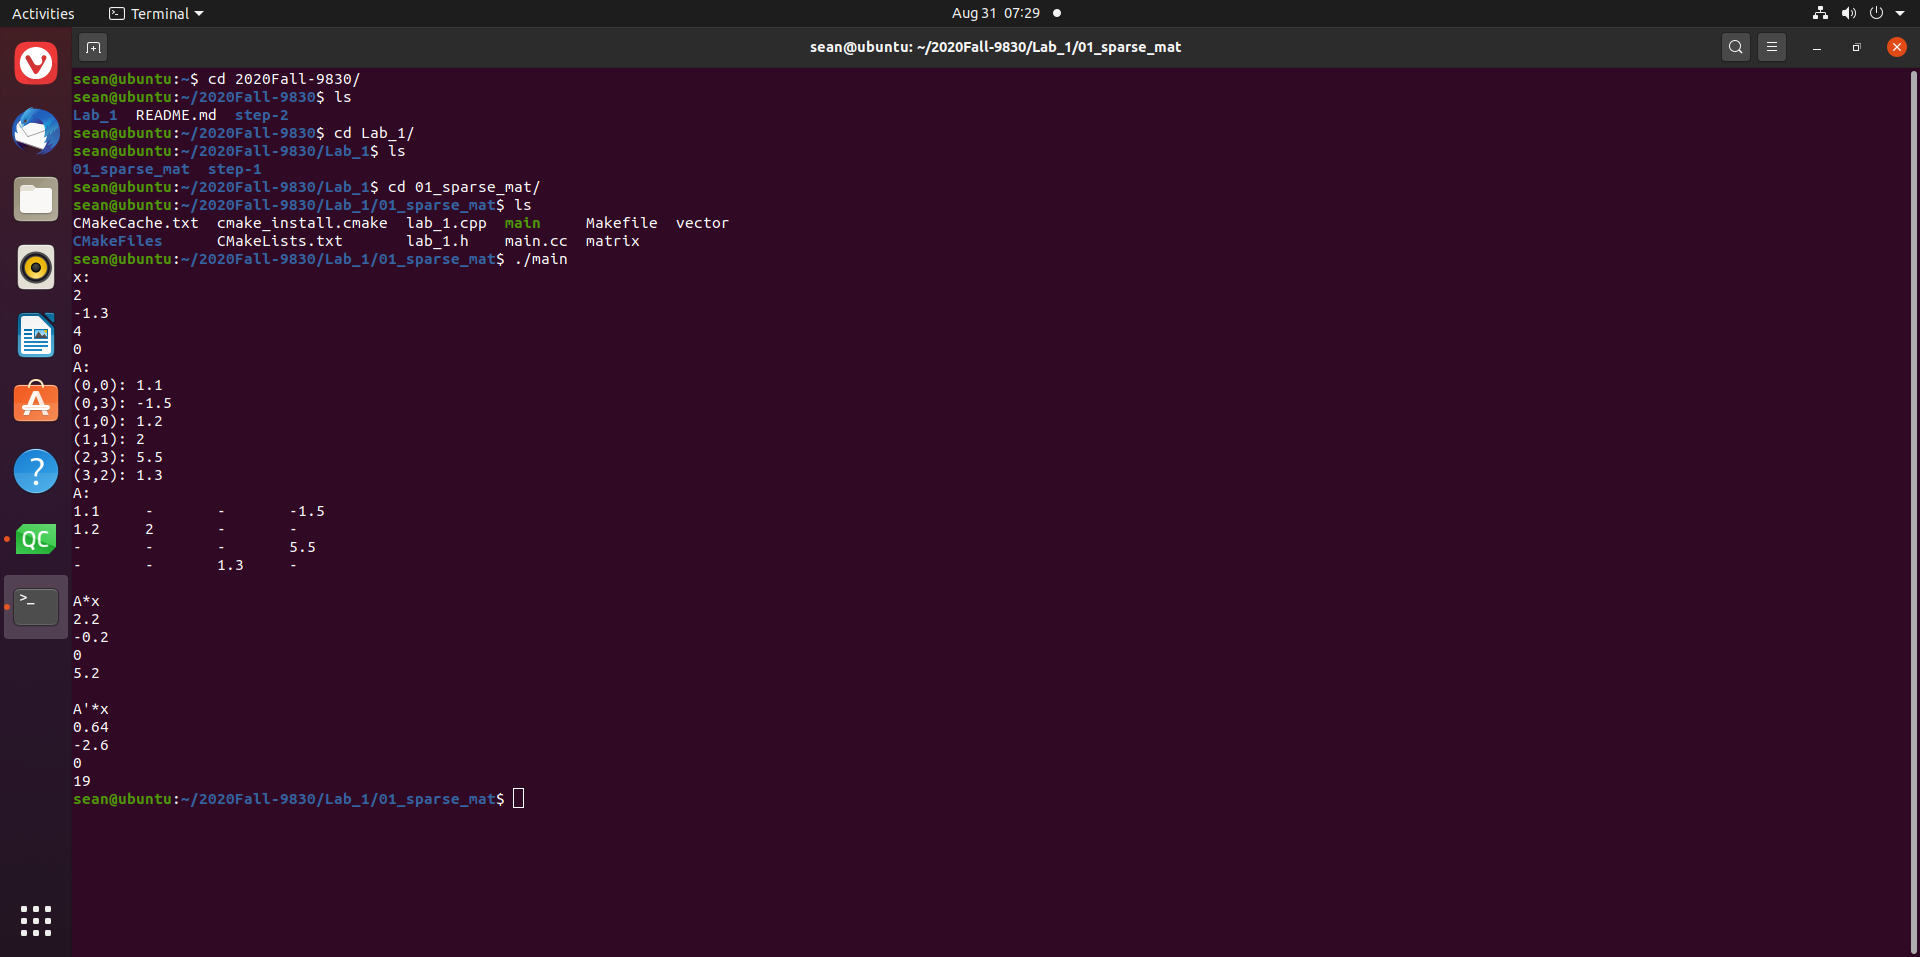
\includegraphics[scale=.2]{Prob_3_Screenshot.png}
\label{fig:Screenshot}
\caption{Screenshot of deal.II output}
\end{figure}
\end{tcolorbox}

\item Install deal.II version 9.2.0 on your computer.  See the lecture and Canvas for more information.  Make sure you can run tutorial \texttt{step-1} from deal.II.

\begin{tcolorbox}[breakable]
I've provided a screenshot of my deal.II output in figure \ref{fig:Screenshot}, so that should be enough justification that I've installed it.  Below I will provide the output from \texttt{step-1}:
\begin{figure}[H]
\centering

\includegraphics[scale=.2]{grid-1.png}
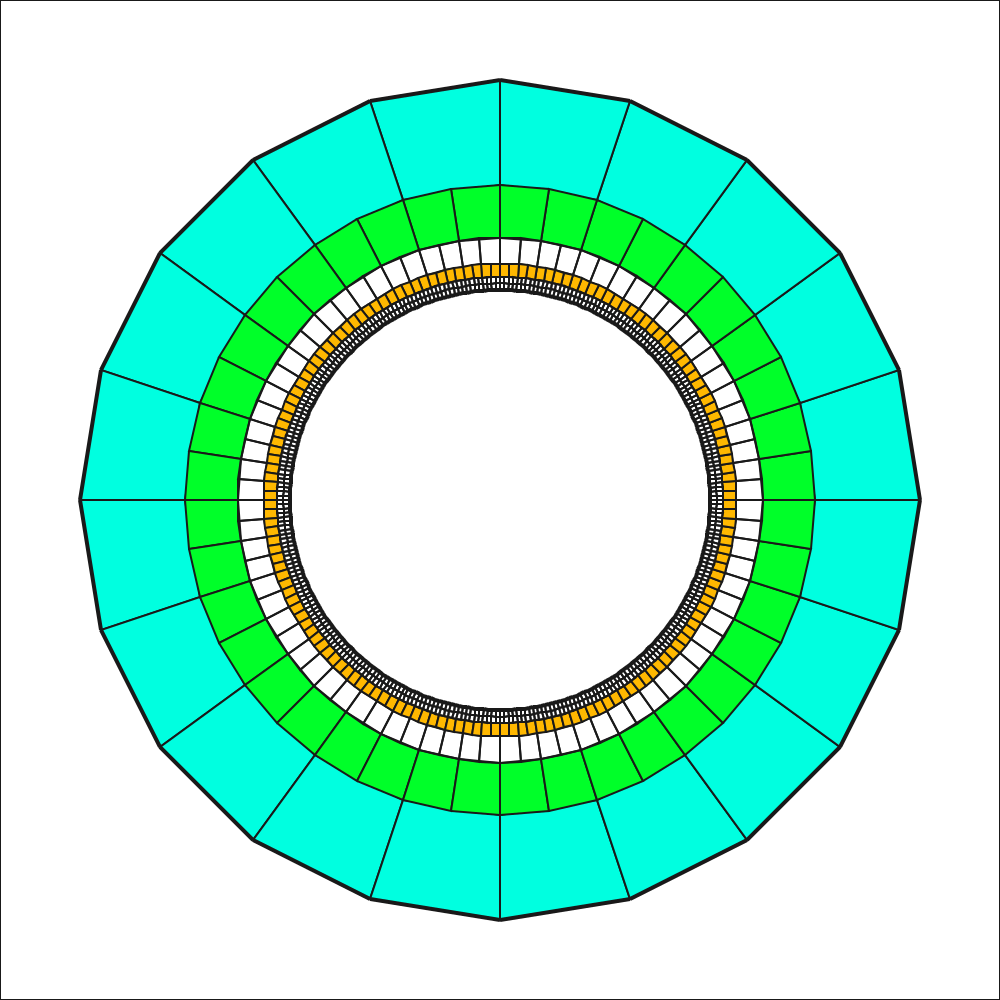
\includegraphics[scale=.2]{grid-2.png}
\caption{Figure 1 and 2 respectively from \texttt{step-1}}
\end{figure}
\end{tcolorbox}
 	

\end{enumerate}
\end{document}